\documentclass[a4paper,10pt]{extarticle}
\usepackage[english]{babel}
\usepackage[utf8]{inputenc}
\usepackage{fancyhdr}
\usepackage[a4paper, portrait, margin=2.0cm]{geometry}
\usepackage{multicol}
\usepackage{paralist}

\usepackage{graphicx}
\graphicspath{ {./}  }

\usepackage{appendix}
\usepackage{listings}

\begin{document}

\begin{center}

\textbf{Python for Business}

\vspace{0.5cm}
\textbf{Motivation, Historical Methods, and Literature Review of RL and its Applications}
        
        \vspace{1.0cm}
        {AUTHOR: Xu Ren}

        \vspace{0.25cm}
        \textit{P4 - April 2020}

        \textit{INSEAD - Singapore}

        \textit{Professor Philip M. Parker}

        \vspace{0.5cm}

        \begin{abstract}
        \section{Executive Summary}
        \noindent
        By convention, the field of machine learning is usually categorized into three major pillars; supervised, unsupervised, and reinforcement learning. It is my opinion and experience that much have been written (both academic literature as well as practitioner documentation) on supervised and unsupervised. As a former data engineer, my own experiences confirm this, over 80\% of work have been in preparing data pipelines for supervised use cases and the remaining being unsupervised. However, I have never encountered the domain of reinforcement learning in my own experiences, yet this appears to be one of the most exciting and rapidly advancing fields of machine learning application in recent years. 


        \bigskip
        \noindent
        Since I worked in a technical function previously and do not come from a strongly aligned business vertical, I will pursue this overview research from a broad look at the field of reinforcement learning, precisely because I feel both under-informed and under-exposed to this branch of machine learning. 


        \bigskip
        \noindent
        We begin by building a motivation for exploring this field and by establishing a parallel historical perspective, particularly of how we thought of artificial intelligence from the early ``rules-engines" days to optimization machines to the more horizontal learning agents they have become today through advancements in computing power and network architectures for deep reinforcement learning. In doing so, we will take a look at packages such as 
        \begin{lstlisting}
        sympy (for formal logic solver in Python)
        scipy and PuLP (for linear programming)
        KerasRL, ChainerRL, pyqlearning, and Tensorforce (for deep reinforcement learning)
        \end{lstlisting} 

        \noindent
        We will conclude with a brief review of how these techniques have been applied across verticals from finance to marketing, and supply chain operations to natural language processing.

        \bigskip
        \begin{description}
        % \item[Usage]
        % Secondary publications and information retrieval purposes.
        \item[Keywords]
        Formal Logic, Constraints Problem, Optimization, Linear Programming, Q Agents, Policies, Rewards, Deep Reinforcement Learning, Recurrent, Exploration and Exploitation
        \end{description}
        \end{abstract}

        \end{center}

        \vspace{1.0cm}
        \begin{center}
            \textbf{Body}
            \end{center}

            \begin{multicols}{2}
            [
            \section{Introduction and Motivation}
            Nearly eight years ago, I was, as with many 22-year-old's, in a semi-delusional state while sitting in a cold university classroom, along with rows of many other students, taking the LSAT exam. For those who are fortunate enough not to know what the LSAT is, it stands for the Law School Admissions Test and is the law school equivalent of the GMAT. One of the most interesting parts of the LSAT is a riddle-like section that tests you on formal logic with obscure situations such as A, B, and C are trying to go to a party but if and only if it is not raining and if A goes then B does not go, etc. Now, under normal circumstances, without the adrenaline-induced heart attacks of a timer, I actually quite enjoy these puzzles. However, with only about a minute to solve one in testing environments, I found that to be rather useless in judging my logical reasoning skills and above all, even then, I found it futile whenever I thought to myself, surely a machine can solve this in a few milliseconds?
            ]

            \subsection{Brief History}
            Fast forward to today, this nearly a decade-old conundrum still interests in me, and I would like to explore how the nature of logic, riddles, and games have influenced our thinking about artificial intelligence and how we have evolved computational methods to these type of problems, such that many are being used in production to solve large-scale enterprise applications. 

            The fascination with ``machines that can think" is nothing new, spanning back from various origins that range from decades to centuries. For the sake of this paper, we will limit it to roughly the 1950's - when the term artificial intelligence was coined. However, the computing power of that time simply could not handle the type of high-dimensional processing that we can achieve today to make algorithms usable and generalizable. 

            This led to a somewhat lull in the advancements in machine learning applications and artificial intelligence. What did come out of this era was the rise of expert systems or sophisticated rules engine, essentially decision branching machines that could navigate paths of conditions far faster than any human could. This is where I will start with my exploratory research, driven by my motivation of LSAT formal logic problems. From here, we will advance to the next phase of machine advancement, which was to use computers for optimization and simulation; particularly, I will look into the area of linear programming for optimizations. 

            With these type of optimization and simulation techniques, machines became exceedingly skilled at exhausting probabilistic landscapes, exploring and evaluating functions repeatedly and finding best actions given its ability to store all possible actions in a finite world. However, something rather stunning happened around the mid-2000's.

            In 2005, Roger Mougalas from O'Reilly coined the term, Big Data. While there are many soundbite definitions of big data, I will subject the scope of this paper to the meaning that big data is a relative term that simply denotes a physical limit whereby the dataset cannot fit on a single machine, or even more precisely, cannot realistically fit into memory of a single machine. For me, this is extremely important and its importance is augmented  by the fact that the world was also simultaneously experiencing a significant drop year-over-year on the cost of hard drive storage and memory chips in general. We began to recognize the limits of exhausting all possible scenarios when a combinatorial explosion of potential input data was so massive that no machine in the world could hold it all in memory, much less explore its entire decision space. 

            Thus, instead of programming the rules for decisions and constraints, we moved away from closed-ended linear programming to a more dynamic form of programming, as our problem space became more sophisticated and our computation power also increased rapidly. First, we start in 1990 when Q-Learning, a form of open-world, reward driven, model-free type of reinforcement learning whereby a reward value is assigned for each state transition, such that getting closer to an end goal has a higher Q value while a state transition away from the end-goal may be "punished" with a lowering of the Q value. 

            Much has changed the world since 1990, when I was born, to the year 2016, when I was standing in Philadelphia, watching a replay commentary of Lee Sedol and DeepMind's AlphaGo. As noted earlier, big data was becoming increasingly widespread and the AI community continually thought about how to train an agent that can play the ancient board game of Go (or weiqi or baduk depending on your country) when an exhaustive approach was not possible. It is said that all permutations of moves in the game Go would result in a number greater than the number of atoms in our universe - fitting value functions for all these moves was simply not feasible. 

            The result of this is the application of artificial neural networks with reinforcement learning techniques, created by DeepMind in 2014. The team used artificial neural networks to approximate value functions of the reward policy for a limited number of forward-looking moves given the current state, such that the algorithm fits on a single machine. The team also introduced a form of training known as experience replay, such that AlphaGo can learn from previously played human matches as well as replay matches over and over without the assistance of a human player. 

            This was a major leap in the advancement of reinforcement learning for the AI community, and the state of the art of this domain continues to be pushed today. Next, we will see some Python specific libraries that cover the scope of the history we just laid out here and conclude with some business verticals that have live use cases for reinforcement learning. 

            \smallskip

            \end{multicols}



            \begin{multicols}{2}
            [
            \section{Evolution of Techniques and Python Implementation}
            In this section, I will present some of the existing libraries and implementation methods for formal logic problems, constraints problems, optimization problems, and an overview of the field of reinforcement learning and deep reinforcement learning. 
            ]

            \subsection{Formal Logic Machines}
            Going back to my initial LSAT conundrum, I wanted to explore Pythonic methods for solving formal logic reasoning problems, and it is also a good starting point for understanding the initial use of machines as rules engines. Here, we take a look at the \textbf{sympy} library and its sub-module of formal logic methods. 

            In the screenshot below, we can see that we can declare three entites (such as three individuals trying to go to a party). We can use formal logic symbols and the package even supports pretty printing to LaTeX. We can say things like if A goes to the party, then B does not go. Furthermore, we can chain the rules together such as in cell 7, where C goes if and only if A goes and at least one of A, B, or C goes to the party: 

            \smallskip
            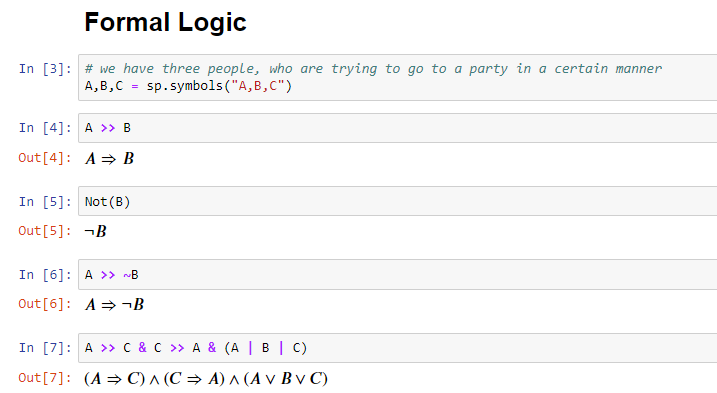
\includegraphics[scale=0.4]{screen1.png}

            \smallskip

            With sympy, we have a method to deduce all of the logic that we must know to be true given the conditions, it is in a sub-module called \textbf{sympy.logic.inference.satisfiable}.
            We can use staisfiable to create an iterable of all possible solutions. 

            \smallskip
            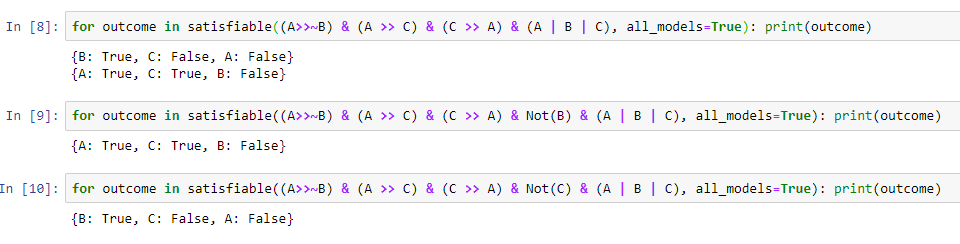
\includegraphics[scale=0.3]{screen2.png}

            And with this one function, we can now answer a question such as C goes to the part if and only if A goes to the party, but if A goes to the party then B does not go, and we are given the factual statement that C does not go. Thus, we have a single solution that only B goes to the party. 

            \smallskip

            \subsection{Constraint Programming}
            Most of the times, the logical reasoning problems on standardized tests, save for a sample of the first few problems, are usually not just formal logical deductions, they tend to be a bit more sophisticated around constraints, such as seating four people in a row of four seats. Here, we can use a python library called \textbf{python-constraint}, and we can create a problem object and add variables of the decision space to it. For example:

            \smallskip
            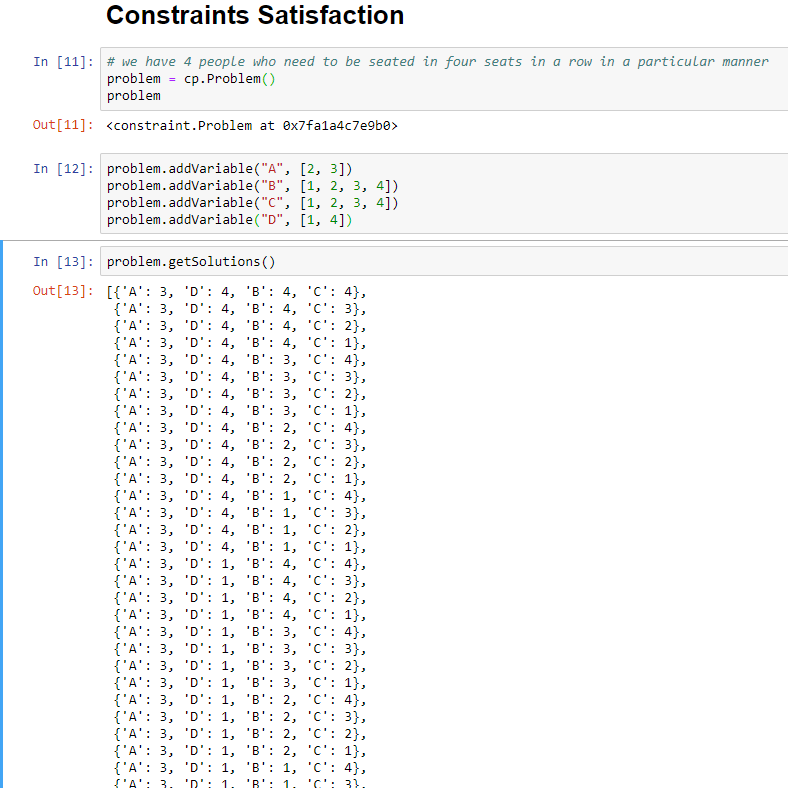
\includegraphics[scale=0.35]{screen3.png}


            \noindet
            Here, we state that person A cannot sit at the ends of a row of four seats and that person D can only sit at the ends. Persons B and C can sit anywhere in the initial problem space. With this, we can see that we have a rather large permutation of potential solutions, so we can start adding our constraints. 

            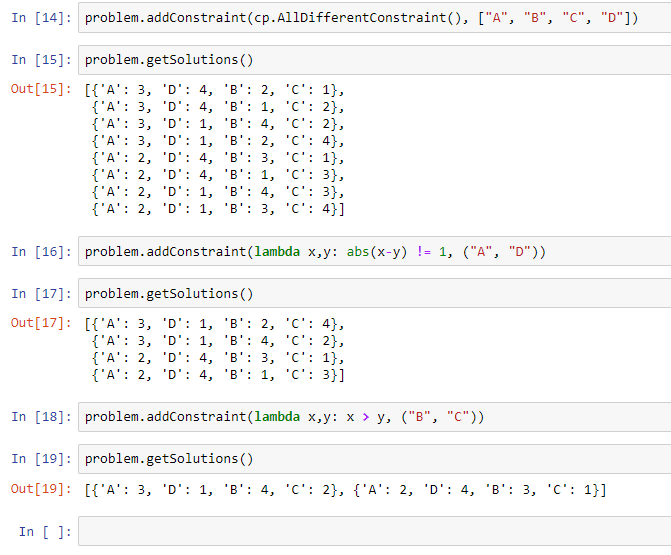
\includegraphics[scale=0.4]{screen4.png}
            \smallskip

            Intuitively, we know that two people can share the same seat, so we can add a constraint that all four seats need to be filled by different people, and this reduces are potential solution space significantly. 

            Next, what is really powerful with this package is that we can use lambda functions to dynamically build our constraints, such as the difference between A's seat and D's seats cannot be 1. In other words, A and D cannot sit next to each other. Given our previous constraint and the initial problem space, this reduces A and D's seats to {1,3} or {2,4}. 

            Lastly, we add the constraint B must sit in a seat that is greater than C's seat. Finally, we are left with two unique solutions to our seating arrangements, and we can easily answer a question such as how many ways can you seat four people given these constraints. 


            \subsection{Linear Programming}
            About two years ago, I took the GMAT for business school applications and here, I encountered another type of problem that I enjoyed solving, especially without the stress of time in a testing situation. The general setup is usually something around two machines working at the same time but the two machines produce different outputs per hour and of course require different costs to operate per hour. Given some constraints, we are usually asked to solve (or to estimate) the best number of hours to operate machine 1 or machine 2. 

            Of course, we can usually solve these close-ended solutions with brute force or with systems of equations and even by leveraging shortcuts using linear algebra. However, python libraries are especially well suited for these kind of problems given python's special place in the scientific and numerical computing communities.

            For example, let's set up a problem with two machines, and we have a requirement from management to produce at least 100 bags today:


            \lstset{basicstyle=\tiny}
            \begin{lstlisting}[language=Python]
            # we have two machines
            # m1 makes 10 bags per hour, 
            # m2 makes 12 bags per hour
            # m1 costs $100 per hour, m2 costs $180 per hour

            # cost_fn = 100x1 + 180x2
            # constraint 1: 2x1 + 1x2 <= 16
            # we have a large order, and need to make 
            at least 100 bags today
            # constraint 2: -10x1 -12x2 <= -100


            # setup
            # https://docs.scipy.org/doc/scipy-1.1.0/
            reference/generated/scipy.optimize.
            linprog.html#scipy.optimize.linprog

            linprog(
                c=[100, 180],
                    A_ub=[[2, 1], [-10, -12]],
                        b_ub = [16, -100]
                        )
                        \end{lstlisting}

                        For the output, we can see we find the best allocation of hours for the two machines while satisfying the 100 bags criterion:

                        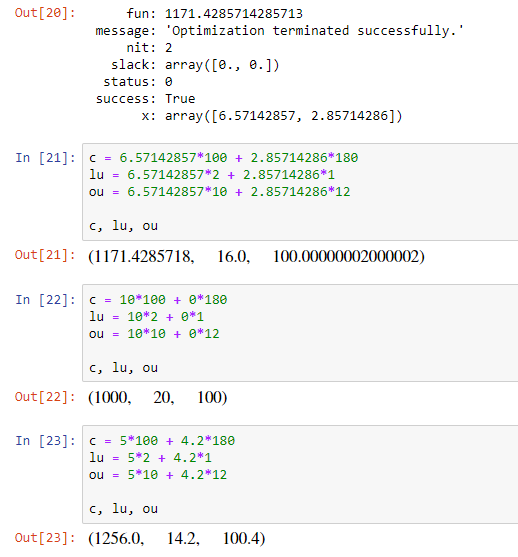
\includegraphics[scale=0.45]{screen5.png}

                        And if we were to use any other combinations of hours, we can see that we either dissatisfy the total number of labor units we have or we result in a higher total cost at the end of the day.

                        For this demonstration, we leveraged the \textbf{scipy} library in python, as this is one of the most commonly used packages in the python scientific universe. If you would like more flexibility in defining constraints and optimization functions, take a look at the \textbf{PuLP} library, designed specifically for linear programming in python.

                        \smallskip


                        \subsection{Modern-Day Reinforcement Learning}

                        \subsubsection{Q Agents}
                        With a much clearer understanding of the history and the implementation of these early techniques, I will now enter into the territory of reinforcement learning, starting with an earlier method known as Q-Learning that originated in 1989-1990. Manually implementing reinforcement learning use cases, as I had done earlier, is quite time consuming and requires that we set up our environments, such as mazes, parking lots, etc. Given the scope and time constraints for this paper, we will simply talk about the theory of these reinforcement learning techniques and then continue into the business applications of such techniques.

                        With Q learning, we essentially have a layout of the world, known as the action space. Next, we have an agent who is allowed to randomly explore this action space, in attempt to reach some end-goal. To know how to get this end-goal and whether the agent is on track, a key part of reinforcement learning is assigning rewards and punishments. The agent will then make many iterations, in the realm of thousands or even millions, and on each iteration, the agent will update its values in its Q network such that for every current state, it updates the values of its next potential actions from that current state. In other words, if the agent is currently standing on block 1 and it can go right or down, it takes a look at its Q network, and sees that going right has a Q reward value of 5 but going down has a Q reward value of 10, it is much more likely to go down in order to maximize its total reward function. 

                        This is where Q learning becomes even more interesting, because it is not deterministic. There is this concept of exploration versus exploitation in Q learning, and I believe this is where it really sets itself apart from all previous techniques. In previous problems that I have outlined and implemented in this paper, we assume there is a deterministic, close-ended solution that the computer can quickly converge on. However, the most optimal solution may not always be the one our hard-coded functions converge on. An agent in Q-learning, in addition to its learning rate, has a $$\epsilon$$  value that is essentially a weighted probability of whether the agent explores a different path in hopes of an even shorter or more rewarding solution to the end goal, or the agent continues to exploit its current path of highest Q values that it has accumulated thus far. 

                        What we are left with after many iterations of training is a Q network that the machine has learned on its own, containing values for every state to action pair such that on any given current state, the agent has learned which next state is the best action to take because it can look ahead to its Q network and see the next maximum value to take.

                        \subsubsection{Deep Reinforcement Learning}
                        However, the traditional use Q-learning has been limited to relatively well-known problem spaces and confined environments, such as mazes and smaller games. One major problem with traditional reinforcement learning is that we need to build key-value pairs for all states and actions in the Q network. This is extremely computationally expensive as the environment scales up with more and more data points. We need a way to limit the dimensionality of the problem space, as well as function approximations rather than incrementally updating every Q value in the data structure. 

                        This is where newer methods in deep reinforcement learning comes into play. Rather than building a set of action spaces for every single state, a deep convolutional neural network tries to approximate the next best action to take given a limited snapshot of the problem space at any given point in time, such as this current move in a Go board or this particular frame in a stream of self-driving car videos. In this regard, deep reinforcement learning is much more expressive and given its more stochastic nature, can model much more sophisticated problems as compared to more traditional RL where the end-goal of a maze or getting a player from point A to point B is precisely defined and rewarded. 

                        There are many python libraries, and growing for that matter, that seek to make reinforcement learning more scalable and reusable. Given my limited exposure to this field, I found all of them to be quite ``blackbox" and difficult to unpack fully in order to understand how policy networks and reward functions are actually been implemented and updated. Some of the top libraries I found are pyqlearning, KerasRL, ChainerRL, and Tensorforce. So far, I have found the documentation and implementation of KerasRL to be quite promising, along with a large community of developers supporting and enhancing it. This is an area of future exploration and deeper understanding. 

                        \smallskip


                        \end{multicols}

                        \begin{multicols}{2}
                        [
                        \section{Applications of Reinforcement Learning}
                        This leads us to how these much more flexible, expressive, and computationally robust deep reinforcement learning methods are used today. 
                        ]

                        \subsection{Business Verticals}

                        \subsubsection{Finance}
                        Perhaps most readily recognizable is the use of deep reinforcement as a trading agent in the field of finance. Deep RL models have been used in actual trading environments as well as more non-fast-moving environments such as portfolio allocation. Trading is quite an appropriate application as any point in time of a stock trade is a state that has previous action states and a finite set of next action steps to take, and the computation can be confined to a set number of look-ahead predictions in order to determine what is the next best action to take in the current state. A lot of major companies like JP Morgan and Goldman Sachs already employ these techniques, specialty shops like Bridgewater and Two Sigma also heavily rely on these methods, and of course, newer entrants that specialize in quantitative trading are heavy users of these algorithms such as Quantopian and WorldQuant.  

                        \subsubsection{Marketing}
                        In the field of marketing, deep reinforcement learning can be applied to everything from dynamic pricing to multi-channel attribution optimization for advertising. Given that we have multiple ad copies, multiple user segments, and multiple channels, there are a lot of ways to the path of conversion. Using a deep reinforcement framework to optimize the probabilities of any one of the next choices for a potential customer can yield to higher sales and lower marketing costs. Perhaps without surprise, major companies in the ad space like Google already use reinforcement learning to optimize its Google Attribution services as well as generating dynamic ads on display exchanges or search engine marketing results. 

                        \subsubsection{Operations and Manufacturing}
                        Just recently, in the domain of semiconductor manufacturing, we learned that Google was employing deep reinforcement learning to run massive number of simulations and exploitation of best chip designs to accommodate for factors such as heating, communication busses, interoperability with other stages of chip design. 

                        \subsubsection{Natural Language Processing}
                        Last but not least, I found a specially interesting use case where reinforcement learning was used to train agents how to generate everything from text summaries, scripts, or even new literature such as articles altogether. In this domain, we know that Microsoft has been conducting deep research into the use of reinforcement learning for a whole array of language processing tasks such as image captioning, text summaries, translations, and even more sophisticated text generation such as sentence structure trees, part of speech policies, etc. 

                        \subsection{Conclusion}
                        The fact of the matter is that the evolution of reinforcement learning has a long and rich history - it did just start in recent years with the rapid open-sourcing of deep learning libraries, or the hype of big data, or even the advancements of chess-playing-bots and vertical stacks of mainframes in the 90's. From my own motivation and fascination with puzzles, games, I attempted to scope a research paper here that takes a broad overview of how these techniques evolved over time and eventually culminated to our current day state-of-the-art techniques in deep reinforcement learning. We concluded with a discussion of the various business verticals that have leveraged reinforcement learning in unique ways. 

                        \end{multicols}

                        \end{document}"
